%!TEX root = ../thesis.tex

\section{Top Fan flips}

We never fan flip a fan flip again. We fan flip to remove large topfans. Say larger than 4.


We flip top fans from last fence upwards. We flip any topfan of 3 edges or larger.

Our flip differs slightly if we encounter a split in the bottom boundary path or a already flipped edge below on the rightmost bottom.

Refer to Figure \ref{fig:fanflip:fanflips} for the different kinds of topfanflips.


\begin{figure}
  \centering
  \begin{subfigure}[b]{0.8 \textwidth}
      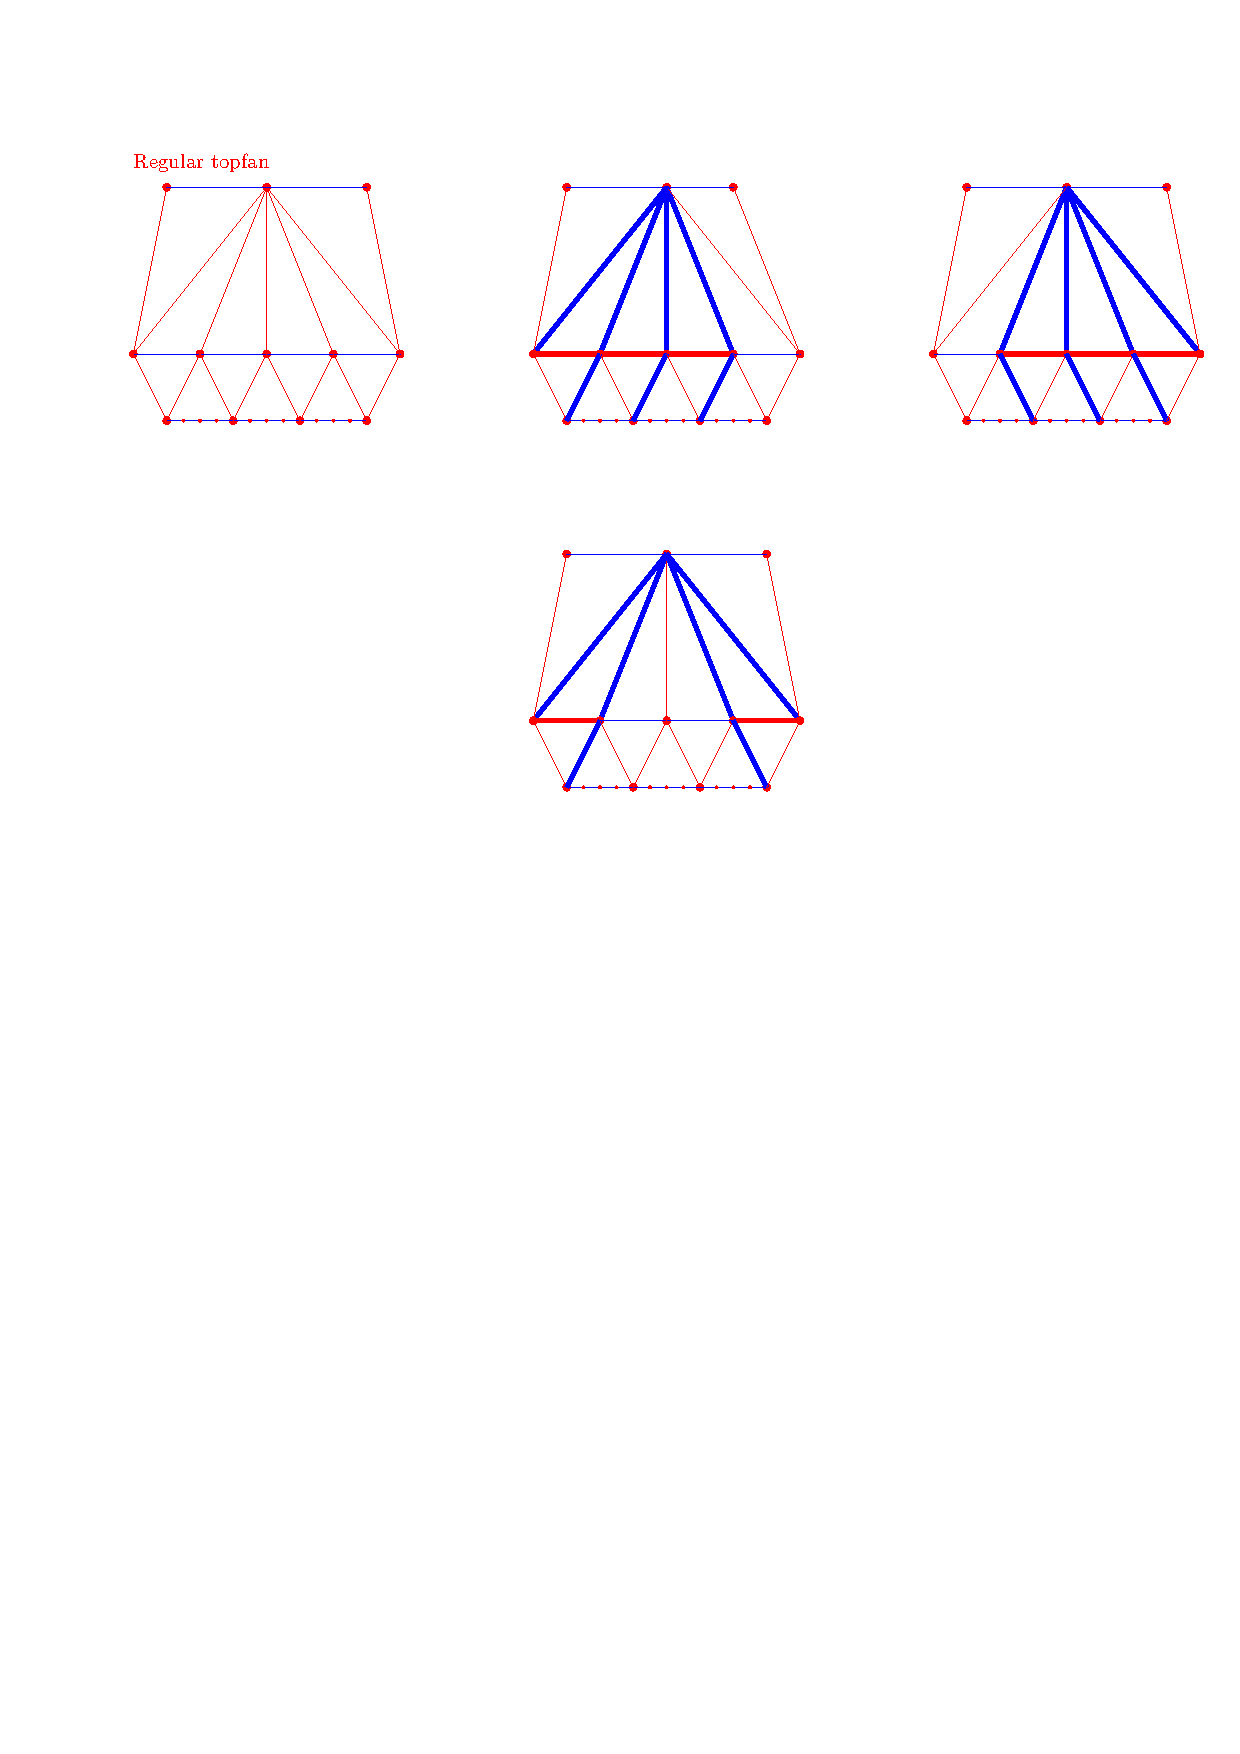
\includegraphics[width = \textwidth]{topFanFlips/img/regular}
      \caption{The regular topfanflip}
  \end{subfigure}
  ~

    \centering
    \begin{subfigure}[b]{0.45 \textwidth}
        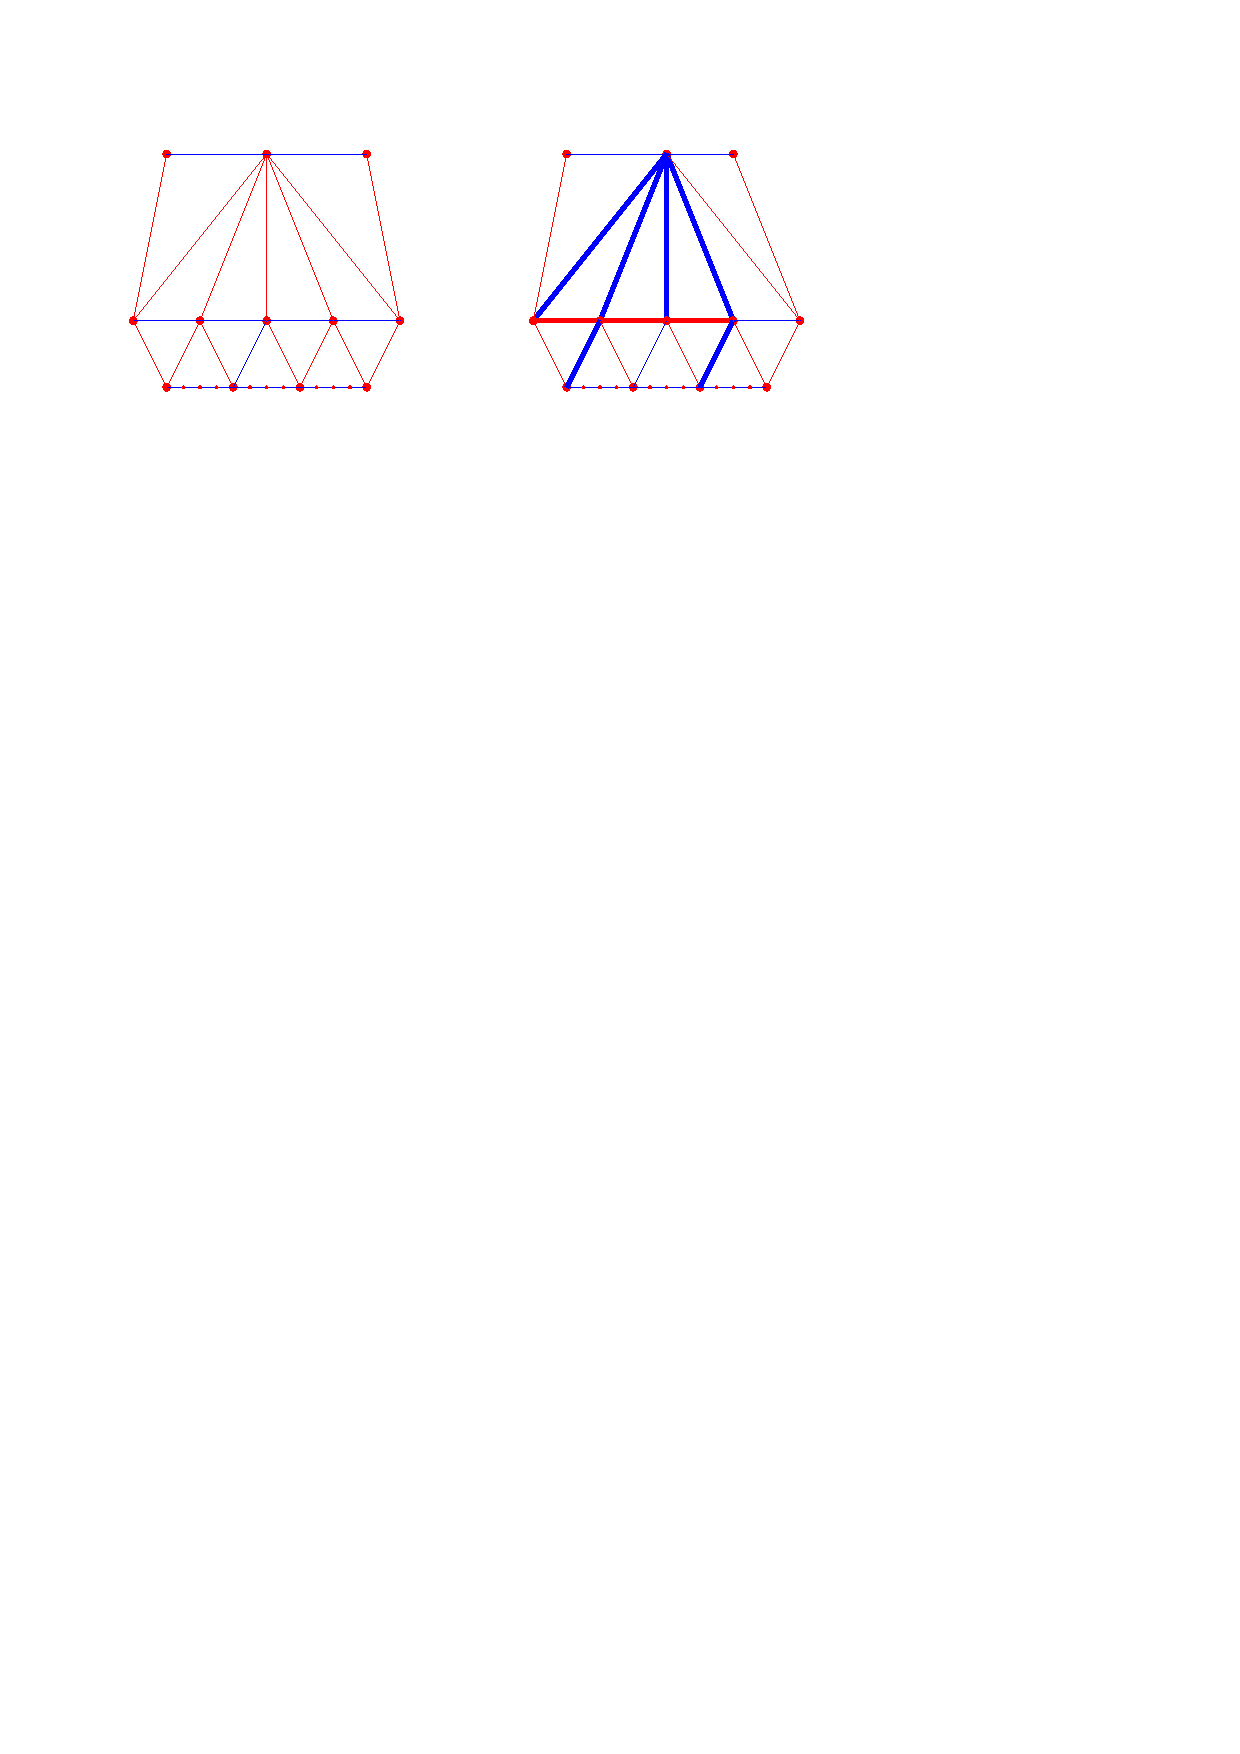
\includegraphics[width = \textwidth]{topFanFlips/img/merge}
        \caption{Topfanflip above a merge}
    \end{subfigure}
    ~
    \begin{subfigure}[b]{0.45 \textwidth}
        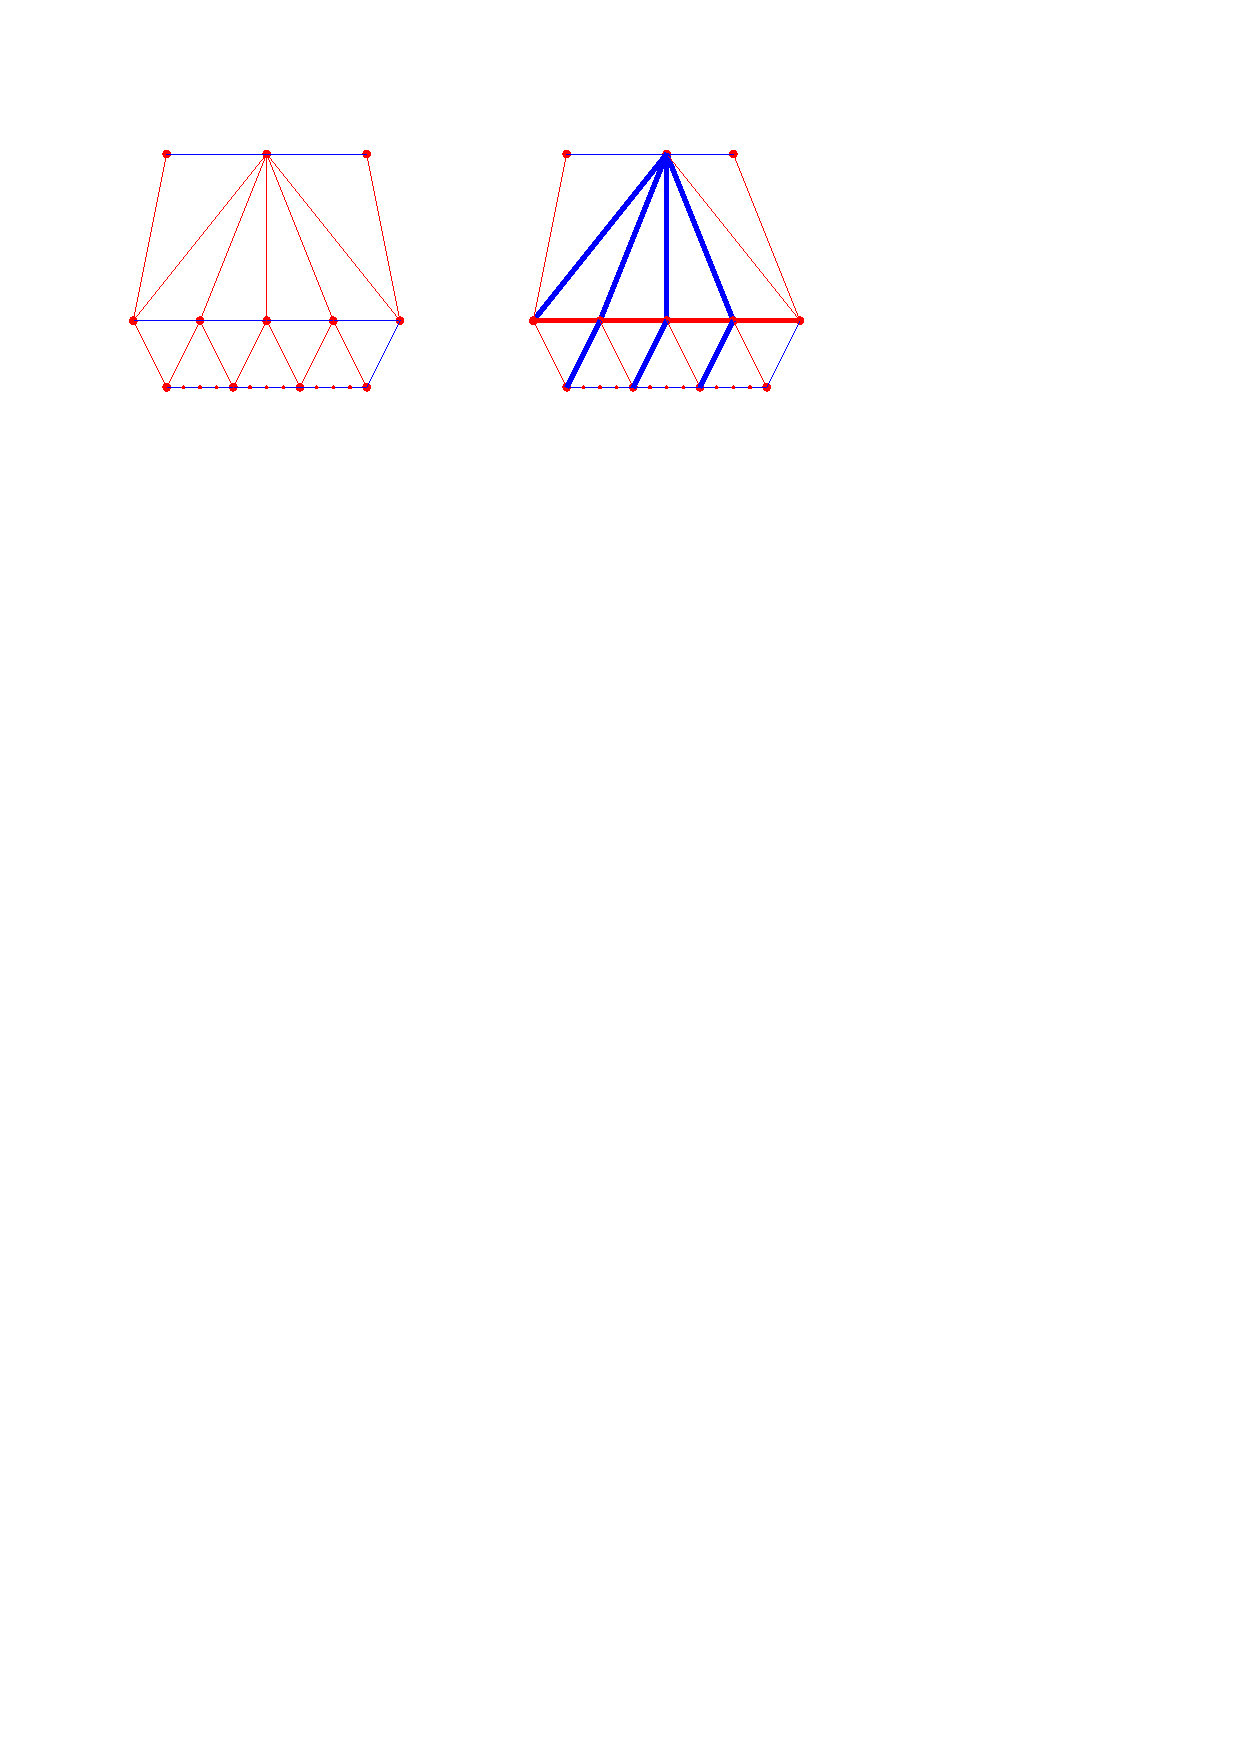
\includegraphics[width =\textwidth]{topFanFlips/img/mergeend}
        \caption{Topfanflip next to merge. Note the additional red edge.}
    \end{subfigure}

    \centering
    \begin{subfigure}[b]{0.45 \textwidth}
        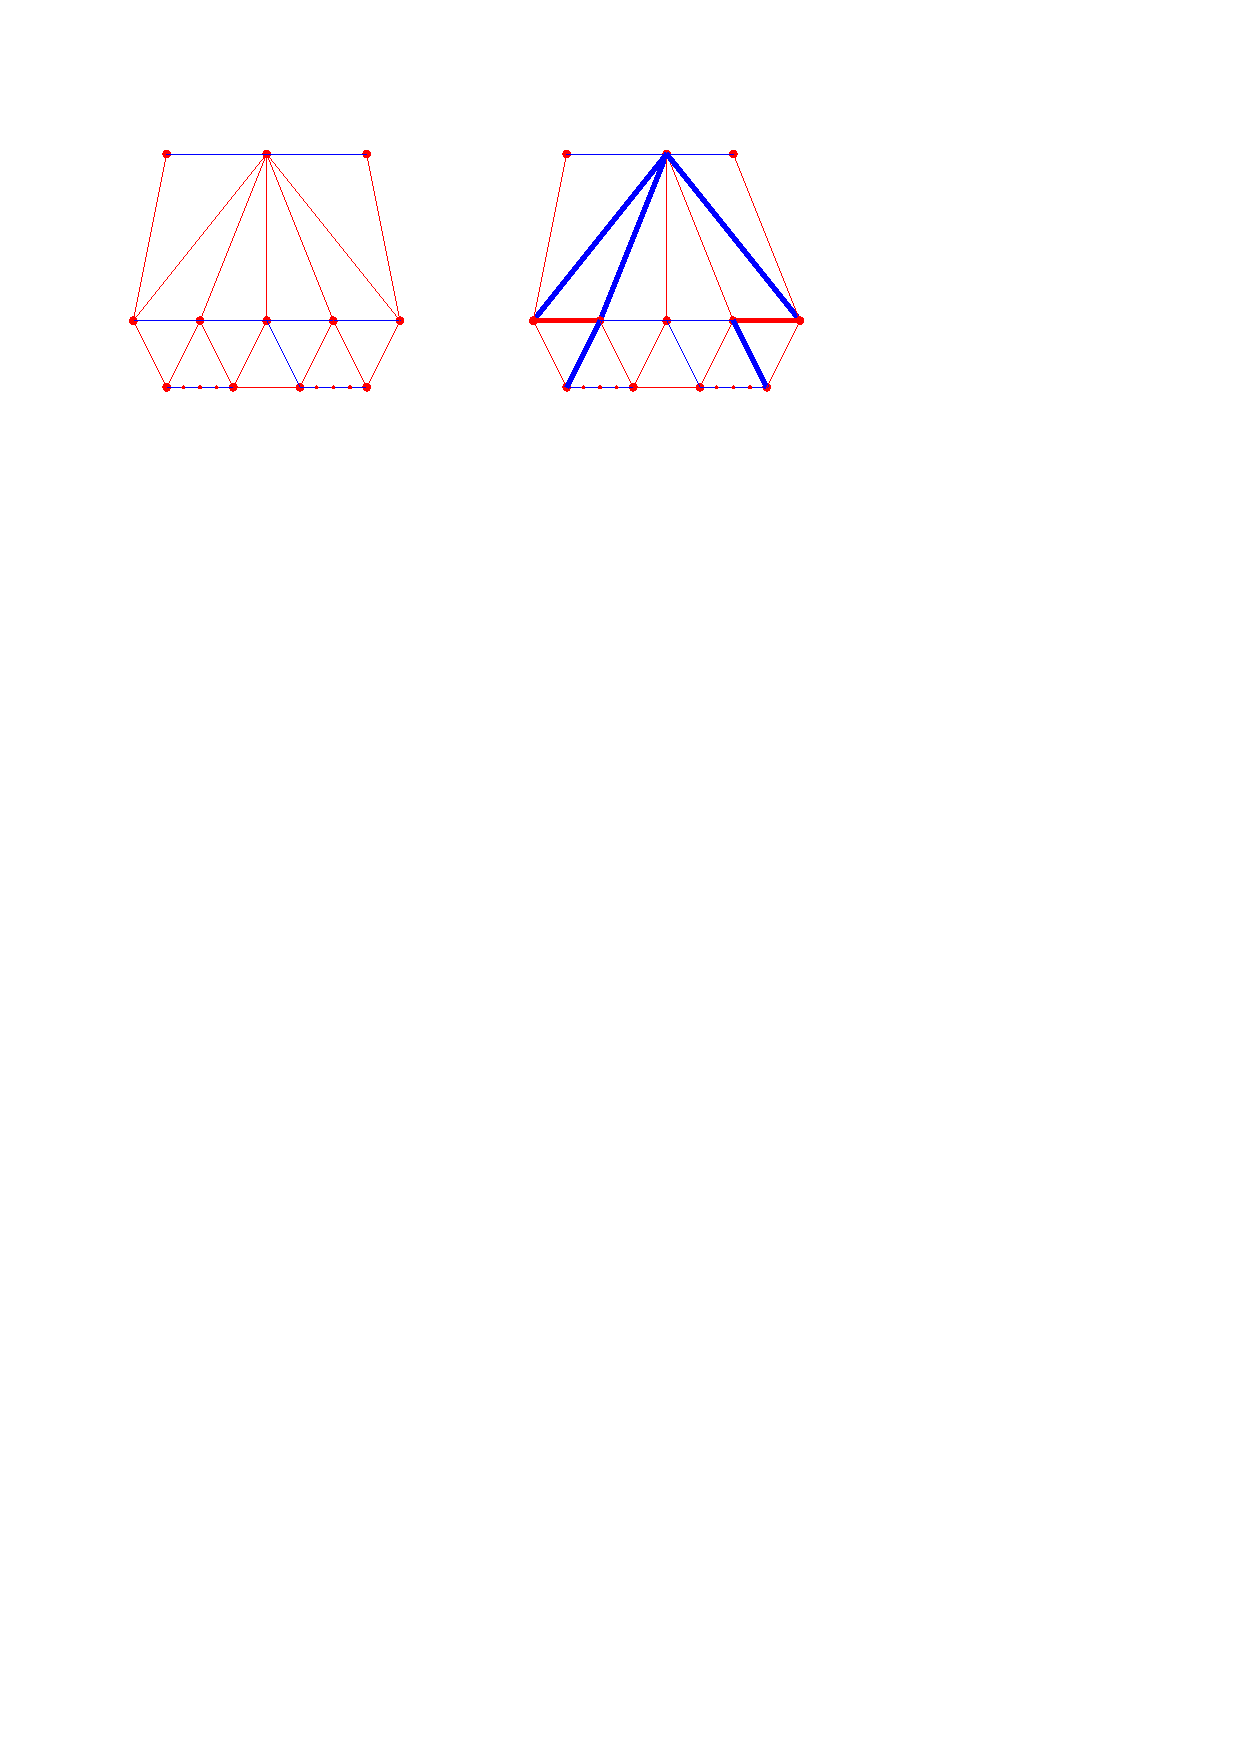
\includegraphics[width = \textwidth]{topFanFlips/img/split}
        \caption{Above a split we stop and we mark the last edge for topload}
    \end{subfigure}
    ~
    \begin{subfigure}[b]{0.45 \textwidth}non
        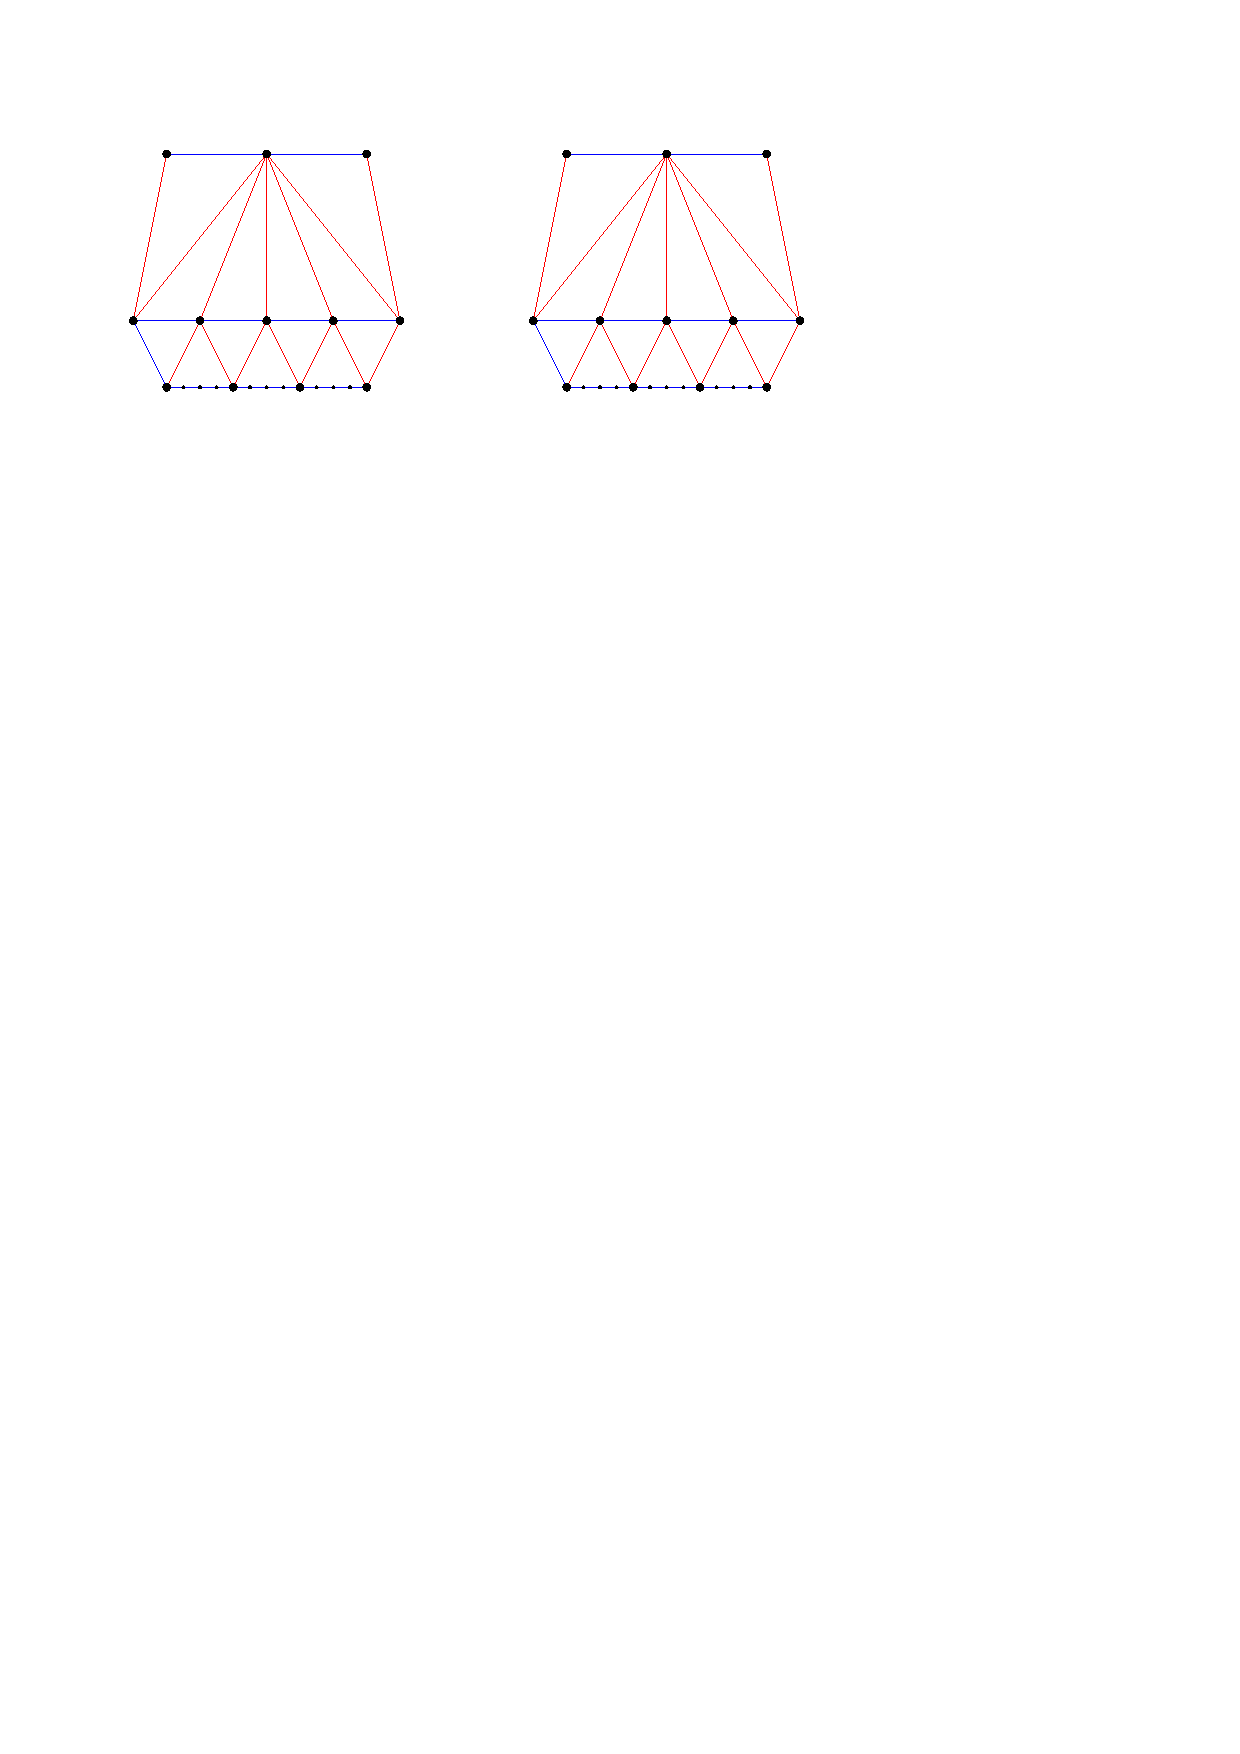
\includegraphics[width =\textwidth]{topFanFlips/img/splitfront}
        \caption{Trouble!}
    \end{subfigure}

    \caption{}
    \label{fig:fanflip:fanflips}
\end{figure}


\paragraph{Description}
When we encounter a topfan we start flipping edges.

We can just flip above a merge. So we do that.

We can't continue flipping above a join. So we don't so this. Instead we mark an edge for potential topload. We will see in the next section how we treat these edges in the next section.


\paragraph{The result}
Befor the topfanflips we had a vertically one-sided REL. After we have a vertically onsided REL. With no large top-fans except at the beginning of faces. Except for the \emph{Trouble!} case.


\paragraph{Trouble}
(If) we can't do anything with the \emph{Trouble!} case  it will increase our bound by $$\max_{(u,v) \in E}   \min\parens{ \deg(u), \deg(v) }$$

We can prove this bound by using  to well-placed chords. \fxnote{We might be able to prevent Trouble! with 3chords. But I'm not sure. I don't think it is straightforward. }

I'm going to ignore this for now.

I guess the other topload can also be very unfortunate. It can even be next to a very large split. So it runs in the same trouble as Trouble.

We kinda want only merges to a certain middle line and only joins afterwards. We can make that transition with topfans. We just can't transition back.
